
%(BEGIN_QUESTION)
% Copyright 2010, Tony R. Kuphaldt, released under the Creative Commons Attribution License (v 1.0)
% This means you may do almost anything with this work of mine, so long as you give me proper credit

Prosesskromatografer er {\it multivariable} instrumenter, og analoge versjoner har derfor ofte flere 4-20 mA-utganger for å sende konsentrasjonsdata for hver målt komponent:

$$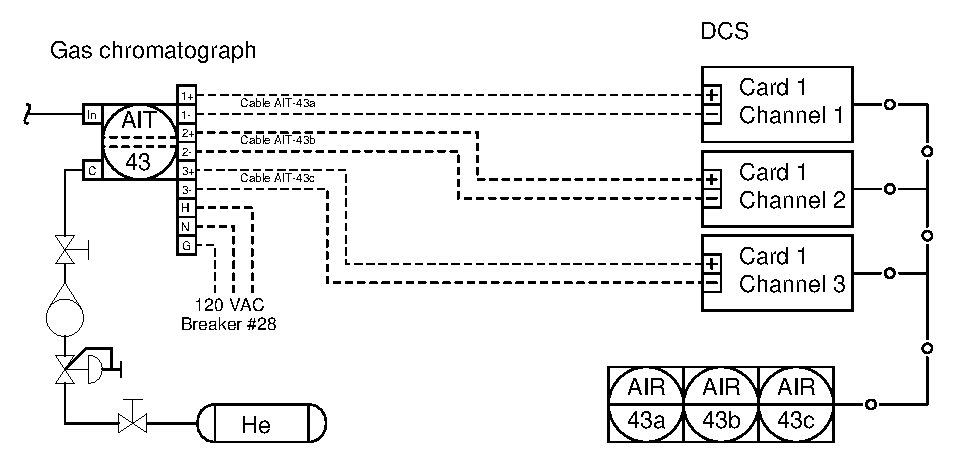
\includegraphics[width=15.5cm]{i00669x01.eps}$$

Se på dette sløyfediagrammet og svar på følgende spørsmål:

\begin{itemize}
\item{} Hva er formålet med beholderen merket ``He''?
\vskip 10pt
\item{} Leverer DCS-inngangskortene 24 VDC sløyfestrøm eller ikke?
\vskip 10pt
\item{} Hvordan ville du koblet en sløyfekalibrator for å simulere et 50\%-signal til AIR-43c?
\vskip 10pt
\item{} Ser du noen måte å redusere antall kabler som trengs for å overføre data fra kromatografen til DCS-et?
\end{itemize}

\underbar{file i00669no}
%(END_QUESTION)





%(BEGIN_ANSWER)

\begin{itemize}
\item{} Hva er formålet med beholderen merket ``He''? {\it Dette er bæregasstanken, fylt med helium.}
\vskip 10pt
\item{} Leverer DCS-inngangskortene 24 VDC sløyfestrøm eller ikke? {\it Mest sannsynlig ikke. Siden kromatografen har egen 120 VAC-forsyning, er det sannsynlig at den er sløyfestrømkilden og ikke DCS-et.}
\vskip 10pt
\item{} Hvordan ville du koblet en sløyfekalibrator for å simulere et 50\%-signal til AIR-43c? {\it Koble fra kabel AIT-43c enten ved kromatografterminalene eller ved DCS-inngangskanalens terminaler. Sett deretter sløyfekalibratoren i "source"-modus (ikke "simulate"-modus) og driv 12 mA strøm inn på DCS-kanalen.}
\vskip 10pt
\item{} Ser du noen måte å redusere antall kabler som trengs for å overføre data fra kromatografen til DCS-et? {\it Bruk digital kommunikasjon i stedet for analog mellom kromatograf og DCS. Ett alternativ er multi-drop HART, et annet er FOUNDATION Fieldbus (eller annen feltbuss som Profibus). Et tredje alternativ er å fjernmontere DCS-I/O nær kromatografen og bruke DCS-nettverkskabel til hovedkontrollrommet. Tilsvarende kan man fjernmontere en PLC nær kromatografen og kjøre nettverkskabel fra PLC til DCS, eventuelt med en "bridge" som oversetter PLC-protokollen til noe DCS-et kan tolke.}
\end{itemize}

%(END_ANSWER)





%(BEGIN_NOTES)


%INDEX% Måling, analytisk: kromatografi

%(END_NOTES)
